\documentclass{article}[9pt]

%%----PACKS----%%
% misc
\usepackage[margin=10pt]{geometry}
% math
\usepackage{amsmath,
            amsfonts,
            amssymb}
% images
\usepackage{graphicx}
% code
\usepackage{listings,
            minted}
\usepackage{inconsolata}
%%-------------%%

%%--SETTINGS---%% 
% minted
\usepackage{xcolor}
\definecolor{cppbg}{rgb}{10,240,240}
\newminted[cpp]{C++}{linenos=true, texcl=true, bgcolor=cppbg, tabsize=4 , frame=lines}
\newminted[bashing]{zsh}

%%--CUSTOM-----%%
\newenvironment{question}
{
\noindent \bf Problem statement. \rm
}

\newenvironment{solution}
{
\noindent \bf Solution. \rm
}

\begin{document}

% authors
\begin{flushright}
	\textbf{Jaap van der Leest\\ Timon van der Berg \\ }
\today
\end{flushright}

% title
\begin{center}
\textbf{C++ Course \\
Assignment 5} \\
\end{center}

%%--BEGIN ACTUAL CONTENT--%%
\section*{Exercise 34}
\begin{verbatim}

1. Differences pointers and arrays
    While the addresses to which a pointer points can be changed, an array will,
    after creation, always be represented by the same block of adresses in memory. 
    This memory is reserved for the array. 
    A pointer does not reserve the memory to which it points. 


2. Differences between pointers and references
    References have to be initialized during decleration and are constant
    thereafter, whereas pointers can be declared without initialization and may be
    changed to point somewhere else after initialization. Pointers can point
    nowhere, references always point somewhere.
    Pointers have to be dereferenced explicitely, whereas references are
    implicitely dereferenced. 
    References can be bound to anonymous values, whereas pointers can not. 

3.
    I suppose tt is a function.

    answer:
    a. int array[20][30] 
    element [3][2] is reached by looking at row 3 and column 2 of an array.
    It is arranged like this:
\end{verbatim}
\begin{figure}[H]
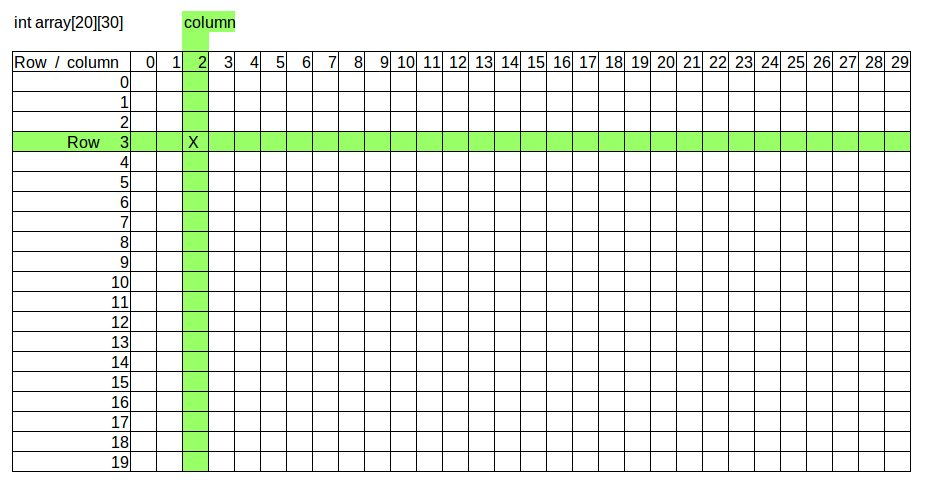
\includegraphics[width=\textwidth]{../34/int_array.jpg}
\end{figure}
\begin{verbatim}
    b. int *pointer[20]
    element [3][2] is reached by taking the pointer to the first element of row 3,
    so pointer[3], then adding 2 to the pointer. C++ knows the size of the element it points to
    so just incrementing the pointer is sufficient to point to the next element, regardless
    of the size of the element in the array.
    this is arranged like this:
\end{verbatim}
\begin{figure}[H]
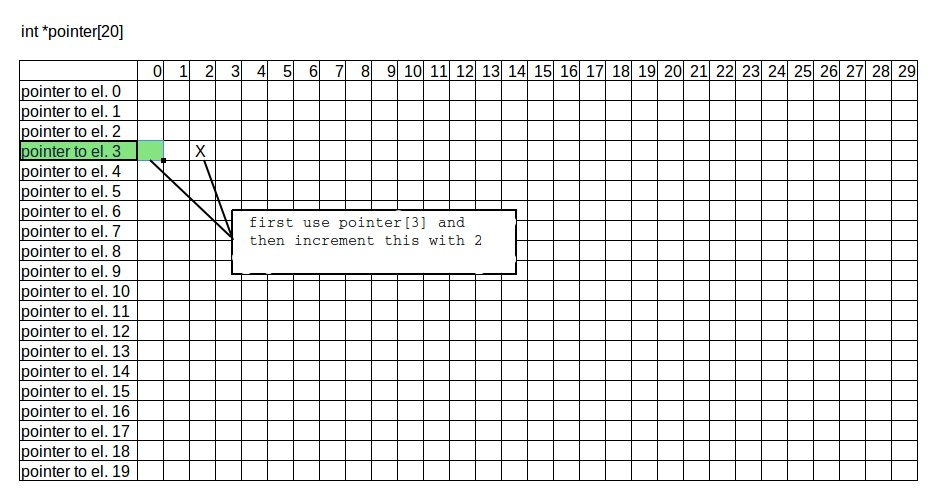
\includegraphics[width=\textwidth]{../34/int_pointer.jpg}
\end{figure}
\begin{verbatim}
    
4. Pointer Arithmetic   
    Incrementing a pointer increases its adress by a value equal
    to the size of the pointer type. This increment ++ptr can be also be written
    ptr = ptr + 1. In the same way we can write ptr = ptr + 3 to move three of 
    <typesize of ptr> to the right. Substraction is defined analogously. 
    Thus pointer arithmetic is just arithmetic on the adress to which the
    pointer points. We can also 
        - compare pointers to pointers
        - compare pointers to 0 or nullptr (pointer that does not point
          anywhere)
        - substract pointer from pointers (tells you how much memory is in between)

5. explain why accessing an element in an array using only a pointer variable is 
   to be preferred over using an index expression.
    the use of pointers is more flexible. 
    e.g. If we want to access a multidimensional array of unknown size this would be
    fairly problematic in a function if we want to give the function the array
    as parameter. Because at the definition of the function we need to know (at least
    part of the) array dimensions. 
    Using pointers we can point to just the start of the array. Giving the function 
    the actual dimensions at runtime it can calculate the appropriate positions of 
    the different values.
    
\end{verbatim}

\section*{Exercise 35}
We apologize for any damage to the eyes of the reader caused by the following table.
\begin{verbatim}
-----------------------------------------------------------------------------------------------------------
definition:         rewrite:             pointers:                    semantics:
-----------------------------------------------------------------------------------------------------------
int x[8];           x[4]            *(x + 4)                          x + 4 points to the
location of the 4th int beyond x. That element is reached using the dereference operator (*)

  int x[8];           x[3] = x[2];          *(x + 3)  = *(x + 2)        x can be considered a
pointer to the first element of the array x. We reach the fourth and third element by pointer
arithmetic.

  char *argv[8];      cout << argv[2];      cout << *(argv+2)           argv is an array of 8
pointers to ints. The cout statement first produces the pointer, i.e. it's adress value. argv
can be considered a pointer to the first pointer in the array. If we increase it by 2 we obtain
a pointer to the third pointer in the array. Dereferencing gives us the pointer in that
position.

  int x[8];           &x[10] - &x[3];       (x + 10) - (x + 3)          x is an array of 8
ints. The & operator here tries to return the adress of the 11th and 4th elements.  The 11th
element does not exist. For a pointer this is 'not a problem', since it will just read the
memory that is there without caring if this is actually part of the array or in fact contains
an int.  What actually happens is the subtraction of 1 address from another. Therefore what is
stored at the addresses is irrelevant in this example. Subtracting the 2 addresses will always
result in 7. 

  char *argv[8];      argv[0]++;            (*argv)++                   argv is an array of
pointers to the first chars of null terminated byte strings.  argv[0] is a pointer to the first
char of the first null terminated byte string.  Incrementing argv[0] means that argv[0] now
points to the second char of the first null terminated byte string. This might be dangerous
because you now have lost a reference to the beginning of the string. So memory leaks can
easily occur.

                                                                        *argv gives the first
first element of argv, i.e. the first pointer in the array. Incrementing means it now points to
to the memory following that char, which also is the second char of the null terminated byte
string.

  char *argv[8];      argv++[0];            *argv++                     argv[0] is processed in
a stmnt. after that argv (so does argv[0]) points to what was argv[1].

  char *argv[8];      ++argv[0];            ++*argv                     first argv[0] (so does
argv) points to the second char in the first ntbs of the array. Then the stmnt is processed.

  char **argv;        ++argv[0][2];         ++*(*argv + 2)              argv is a pointer to a
pointer to a char. In this case it points to the first argument (program name) from that it
points to the 3rd char. The value of this char will be increased by 1. So an A becomes a B.
Thereafter the stmnt is processed.
------------------------------------------------------------------------------------------------------------------------------
\end{verbatim}
\section*{Exercise 36: Strings Class}
The following implements a class \texttt{Strings} wrapping an array of a changable number of std::string elements.
The member functions requested in 37 and 38 are also shown in the class header.
strings/strings.h:
\inputminted[linenos=true, tabsize=4, frame=lines]{text}{../363738/strings/strings.h}
strings/strings.ih:
\inputminted[linenos=true, tabsize=4, frame=lines]{text}{../363738/strings/strings.ih}
main.cc:
\inputminted[linenos=true, tabsize=4, frame=lines]{text}{../363738/main_36.cc}
strings/add.cc:
\inputminted[linenos=true, tabsize=4, frame=lines]{text}{../363738/strings/add.cc}

strings/strings1.cc:
\inputminted[linenos=true, tabsize=4, frame=lines]{text}{../363738/strings/strings1.cc}
strings/strings2.cc:
\inputminted[linenos=true, tabsize=4, frame=lines]{text}{../363738/strings/strings2.cc}
strings/strings3.cc:
\inputminted[linenos=true, tabsize=4, frame=lines]{text}{../363738/strings/strings3.cc}
strings/strings4.cc:
\inputminted[linenos=true, tabsize=4, frame=lines]{text}{../363738/strings/strings4.cc}

\section*{Exercise 37}
See 36 for the class header.
main.cc:
\inputminted[linenos=true, tabsize=4, frame=lines]{text}{../363738/main_37.cc}
strings/at1.cc:
\inputminted[linenos=true, tabsize=4, frame=lines]{text}{../363738/strings/at1.cc}
strings/at2.cc:
\inputminted[linenos=true, tabsize=4, frame=lines]{text}{../363738/strings/at2.cc}
strings/privat\_at.cc:
\inputminted[linenos=true, tabsize=4, frame=lines]{text}{../363738/strings/priv_at.cc}
strings/release.cc:
\inputminted[linenos=true, tabsize=4, frame=lines]{text}{../363738/strings/release.cc}
The filtering is implemented in a class 'filter'.
filter/filter.h:
\inputminted[linenos=true, tabsize=4, frame=lines]{text}{../363738/filter/filter.h}
filter/filter.ih:
\inputminted[linenos=true, tabsize=4, frame=lines]{text}{../363738/filter/filter.ih}
filter/display.cc:
\inputminted[linenos=true, tabsize=4, frame=lines]{text}{../363738/filter/display.cc}
filter/filter1.cc:
\inputminted[linenos=true, tabsize=4, frame=lines]{text}{../363738/filter/filter1.cc}
filter/filter2.cc:
\inputminted[linenos=true, tabsize=4, frame=lines]{text}{../363738/filter/filter2.cc}
\section*{Exercise 38}
main.cc:
\inputminted[linenos=true, tabsize=4, frame=lines]{text}{../363738/main_38.cc}
strings/stringsswap.cc:
\inputminted[linenos=true, tabsize=4, frame=lines]{text}{../363738/strings/stringsSwap.cc}
\section*{Exercise 39}
main.cc:
\inputminted[linenos=true, tabsize=4, frame=lines]{text}{../39/main.cc}
exercise39.ih:
\inputminted[linenos=true, tabsize=4, frame=lines]{text}{../39/exercise_39.ih}
inv\_indentity.cc:
\inputminted[linenos=true, tabsize=4, frame=lines]{text}{../39/inv_identity.cc}
\end{document}

